\anexo{Resultados de la Encuesta}

Se presentan a continuación los gráficos de resultados generados automáticamente por Google Forms, correspondientes a la encuesta de 120 respuestas descripta en el capítulo de User Research (sección de Objetivo de la encuesta, Composición de la muestra y Resultados por segmento).

\begin{figure}[ht]
	\centering
	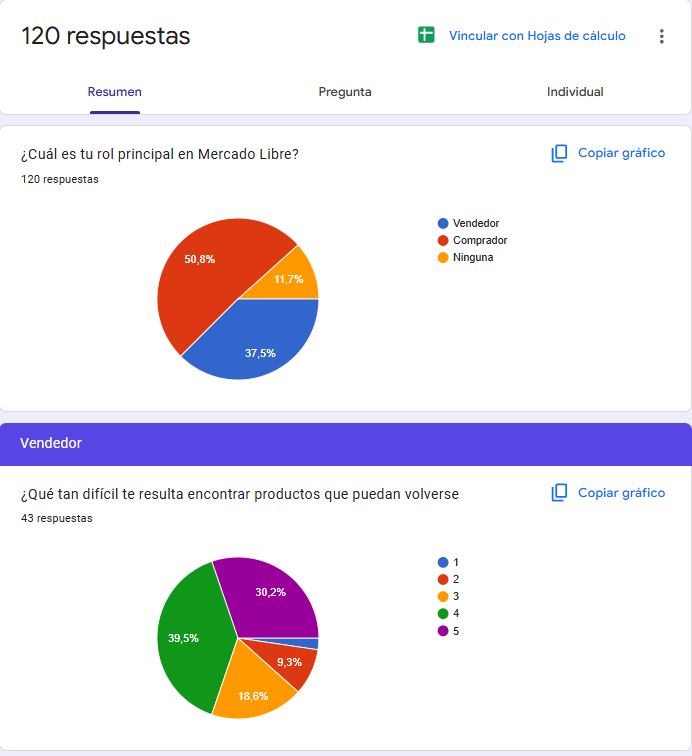
\includegraphics[width=0.68\textwidth]{./images/encuesta/encuesta1Tesis.png}
	\caption{Resultados de la encuesta en Google Forms (120 respuestas, cierre 16/07/2026) -- rol principal y dificultad para encontrar productos en tendencia.}
	\label{fig:encuesta-1}
\end{figure}

\begin{figure}[ht]
	\centering
	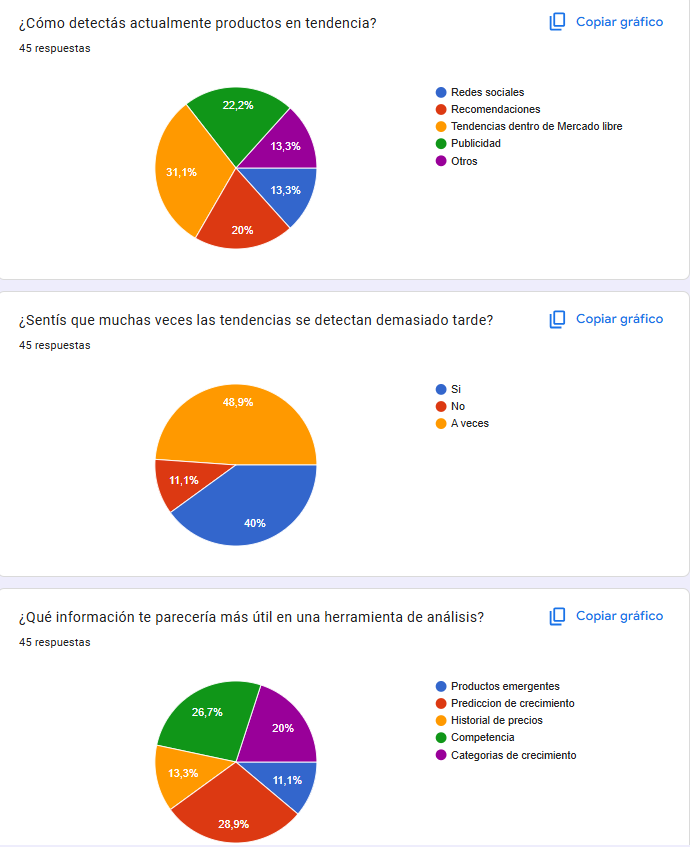
\includegraphics[width=0.68\textwidth]{./images/encuesta/encuesta2Tesis.png}
	\caption{Resultados de la encuesta en Google Forms -- método de detección, percepción de detección tardía e información más útil.}
	\label{fig:encuesta-2}
\end{figure}

\begin{figure}[ht]
	\centering
	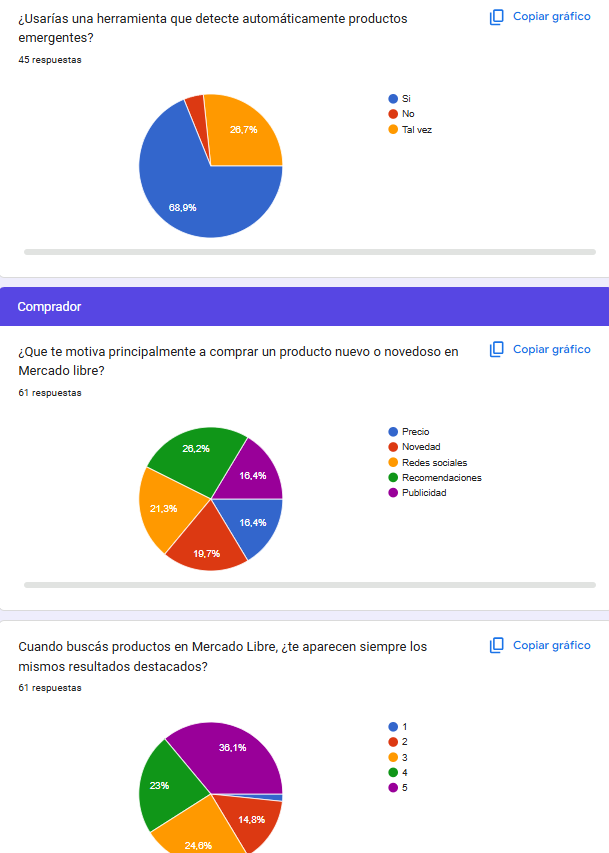
\includegraphics[width=0.68\textwidth]{./images/encuesta/encuesta3Tesis.png}
	\caption{Resultados de la encuesta en Google Forms -- disposición a usar una herramienta automatizada y motivación de compra.}
	\label{fig:encuesta-3}
\end{figure}

\begin{figure}[ht]
	\centering
	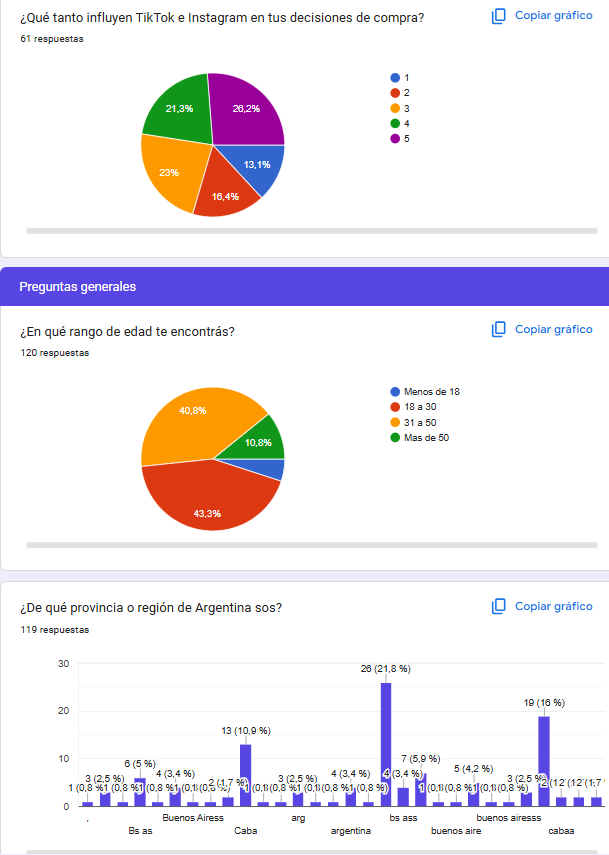
\includegraphics[width=0.68\textwidth]{./images/encuesta/encuesta4Tesis.png}
	\caption{Resultados de la encuesta en Google Forms -- influencia de redes sociales, rango de edad y distribución geográfica.}
	\label{fig:encuesta-4}
\end{figure}